% % % Headers and definitions
\documentclass[10pt]{article}

\usepackage{setspace}
\usepackage{graphicx} % some graphics functions I use 
\usepackage{geometry}
\usepackage{fontspec} 
\usepackage{wrapfig}
\setmainfont{Times New Roman}

\doublespacing
\geometry{lmargin=1in, rmargin=0.5in, tmargin=1in, bmargin=0.75in}
\begin{document}

\pagenumbering{gobble} % Turn off page numbering for titles and tables

% Title and author
\Large{\center{\textbf{{Nick Levesque\\
April 7, 2015\\
ECE 331\\}}}}

\pagenumbering{arabic}
\large
% % % % % % % % % % % % % % %
% Introduction section
\section{Introduction}

\noindent This report describes in detail the design, testing, and validation of the RGB LED kernel module. The module takes three unsigned integers as input, and passes color values to an XMega32E5 on an external board, which drives the RGB LED with pulse-width modulation (PWM) . This module was designed so that multiple processes can open the associated device driver special file simultaneously, with locking used to limit writes to the external board to one process at a time. It is designed for use with all official models of the Raspberry Pi, up to and including the Raspberry Pi 2. 


% % % % % % % % % % % % % % %
% Design and analysis section
\section{Design}
In this section the design details, decisions, and the engineering rationale behind them are discussed.
\subsection{RGB Data}
\noindent To pass color data to the XMega, eleven bits are sent over three GPIO pins (thirty-three total bits in a sequence), with a fourth pin used as a clock. The most significant bits are sent first. In the module's initialization function, these pins are requested from the system and set as outputs with an initial value of zero. The kernel module is passed a struct containing three unsigned integers via an ioctl call. These integers contain the intensity values for red, green and blue. The duty cycle of the XMega's PWM output to each LED pin is high when the LED is dim, and low when the LED is at full brightness. Taking this into account, the module's ioctl handler runs a loop, decrementing a counter, \emph{i} from its initial value of ten until it reaches zero. In each iteration of the loop, the color values are shifted right by \emph{i}. The two's complement of this result is bitwise-ANDed with one, with the relevant GPIO pin being set high if the result is one. The ioctl handler sets the clock high, sets the pins to zero, sets the clock low, then continues looping until finished the sequence.


\subsection{Locking}
\noindent
\begin{wrapfigure}{o}{0.45\textwidth}
    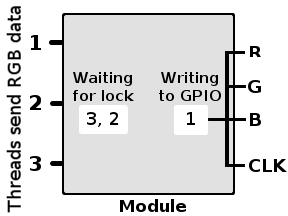
\includegraphics[width=0.45\textwidth]{figure1}
  \caption{Illustration of multi-thread handling}
\end{wrapfigure}
\noindent In order to handle multiple threads attempting to set the LED color simultaneously, only one thread is allowed to write its bit sequence at a time. Mutex locking is used to manage waiting threads. As shown in Figure 1, thread \#1 is currently writing to the GPIO pins, but thread \#2 and \#3 also want to write. Thread \#2 attempted to write before \#3, so it will acquire the lock as soon as \#1 releases it. Thread \#2 will then write its bit sequence, unlock the lock, and thread \#3 will acquire it.

\noindent 

% % % % % % % % % % % % % % %		
% Testing / Validation
\section{Testing and Validation}

\noindent 

% % % % % % % % % % % % % % %		
% Results / Conclusion
\section{Results and Conclusion}

\noindent 

\end{document}
